\documentclass[a4paper,openright,12pt]{article}
\usepackage[spanish]{babel}
\usepackage[utf8]{inputenc}
\usepackage{fancyhdr}
\usepackage{graphicx}

% encabezados
\lhead[\thepage]{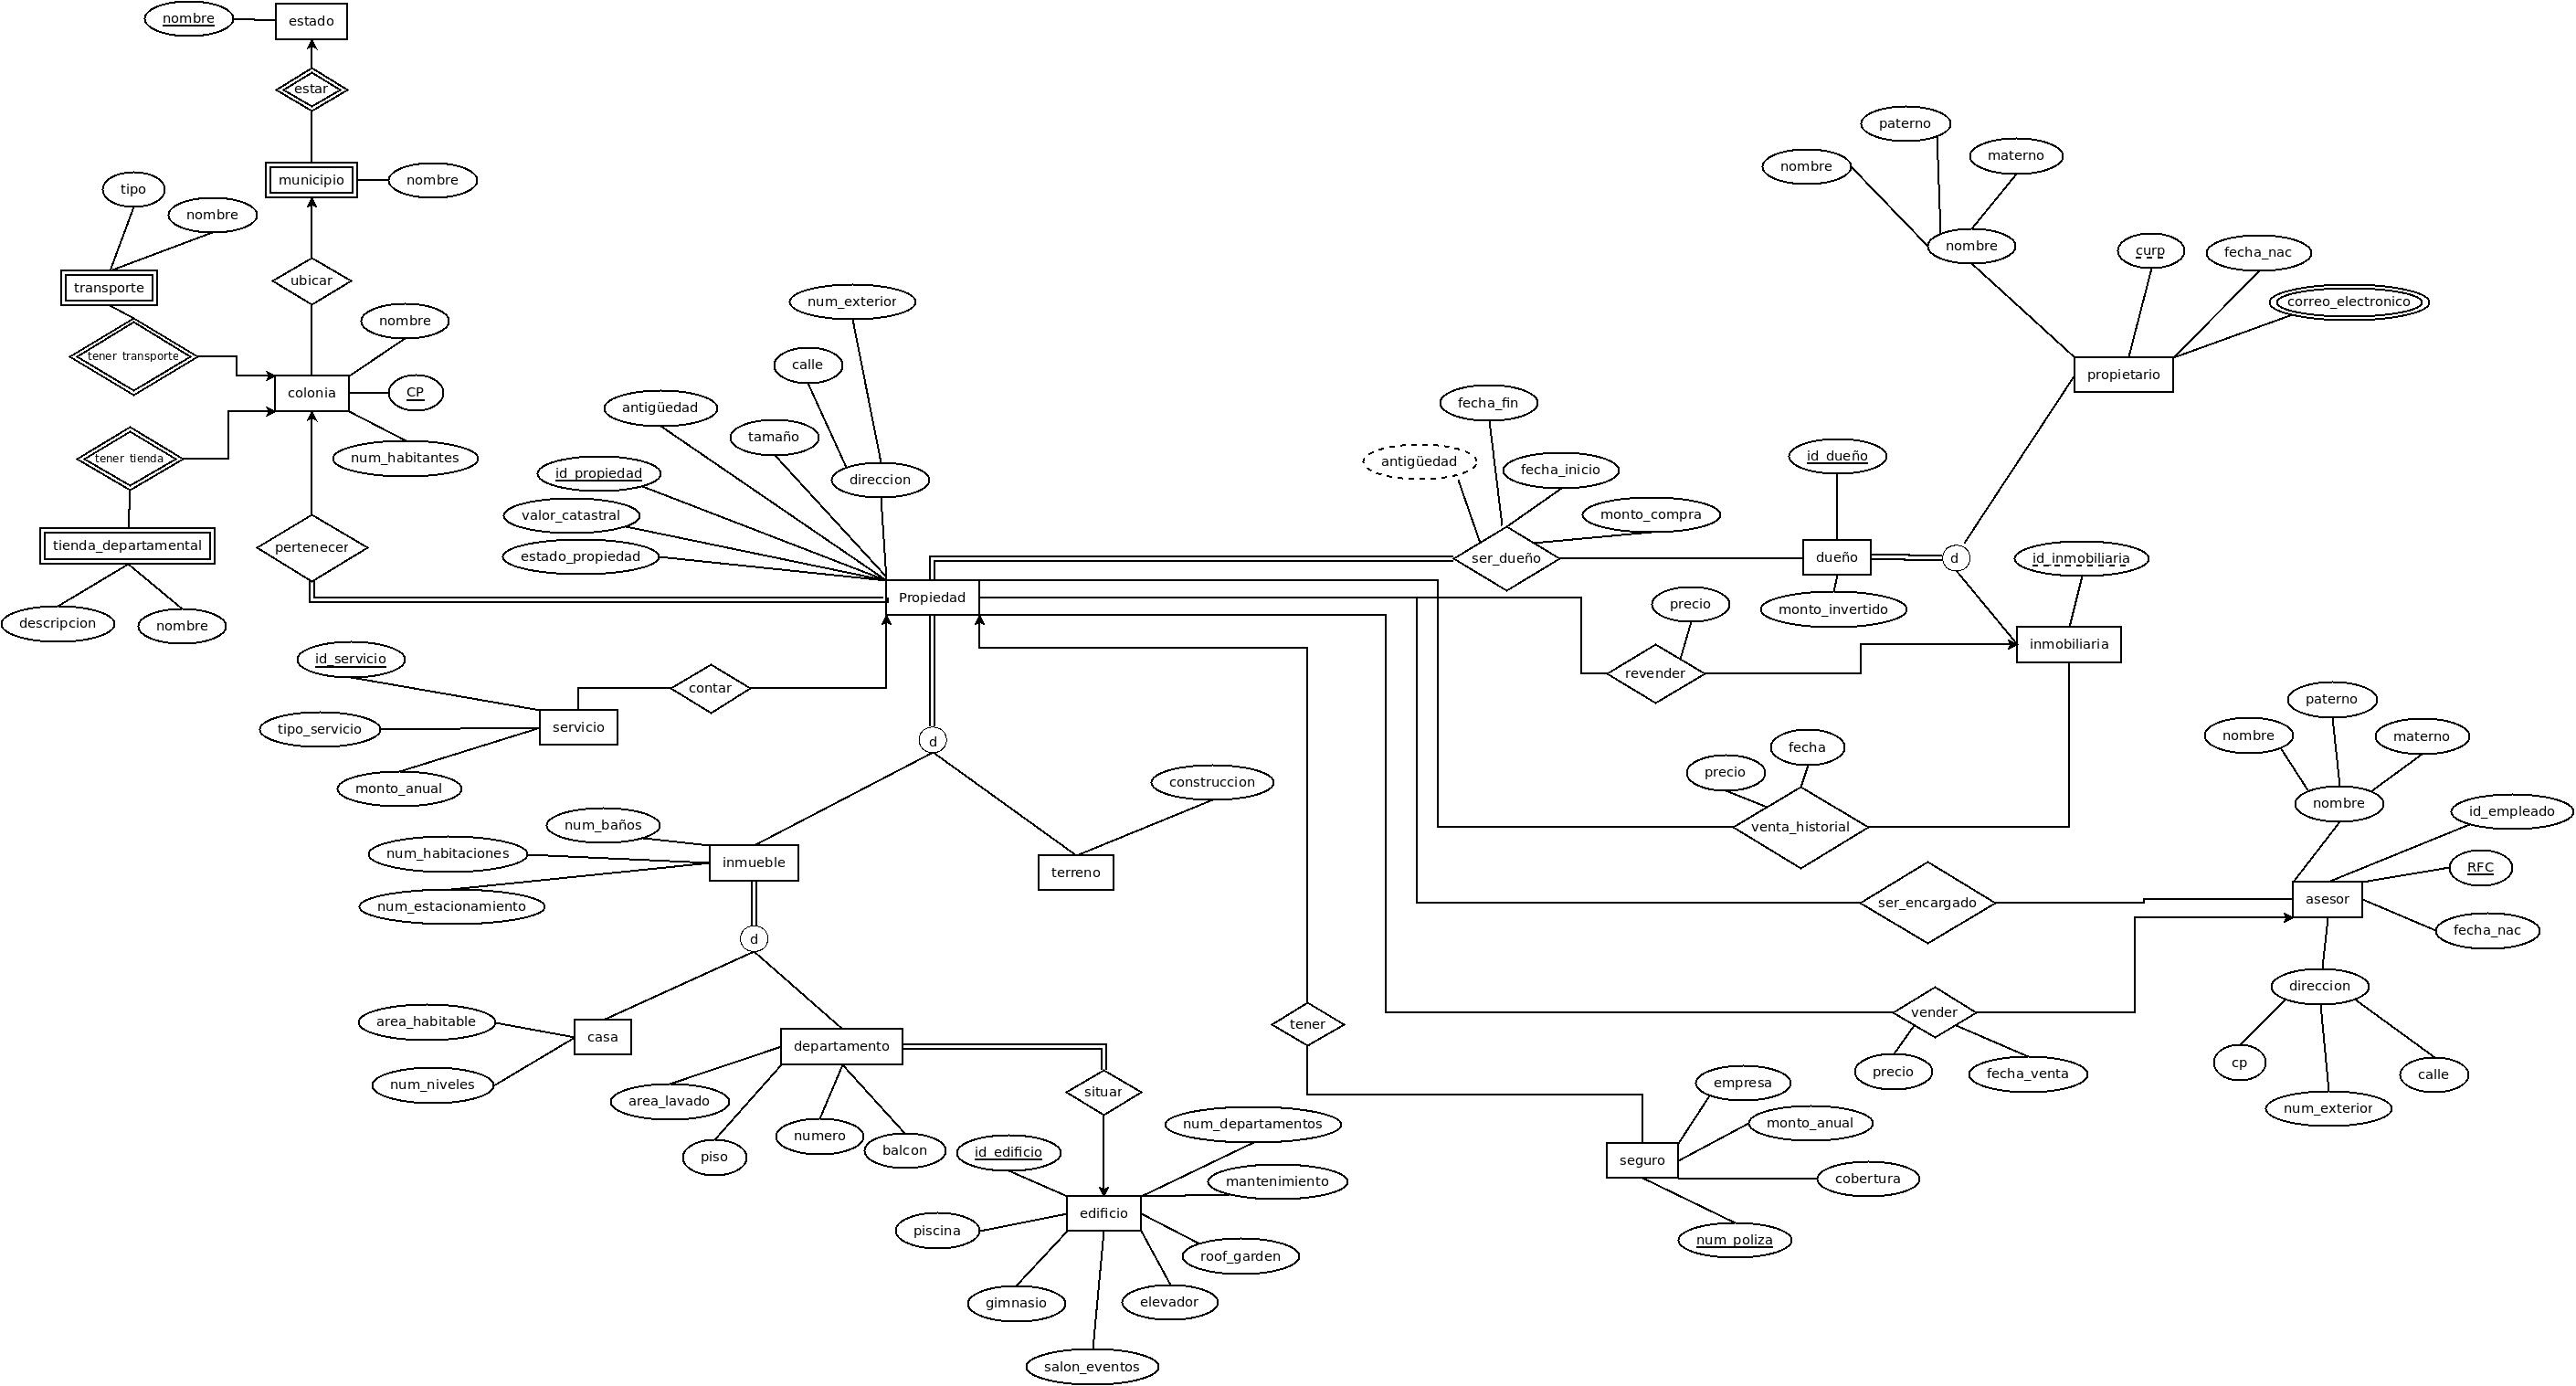
\includegraphics[width=1cm]{modeloER}}
\chead[]{Proyecto}
\rhead[CAPÍTULO \thechapter. \leftmark]{}
\renewcommand{\headrulewidth}{0.5pt}

% pie de pagina
\lfoot[]{\today}
\cfoot[]{}
\rfoot[Arenita Mejillas]{}
\renewcommand{\footrulewidth}{0.5pt}

% primera pagina de un capitulo
\fancypagestyle{plain}{
\fancyhead[L]{}
\fancyhead[C]{}
\fancyhead[R]{\thepage}
\fancyfoot[L]{}
\fancyfoot[C]{}
\fancyfoot[R]{}
\renewcommand{\headrulewidth}{0pt}
\renewcommand{\footrulewidth}{0pt}
}

\pagestyle{fancy}

\begin{document}

\lhead[]{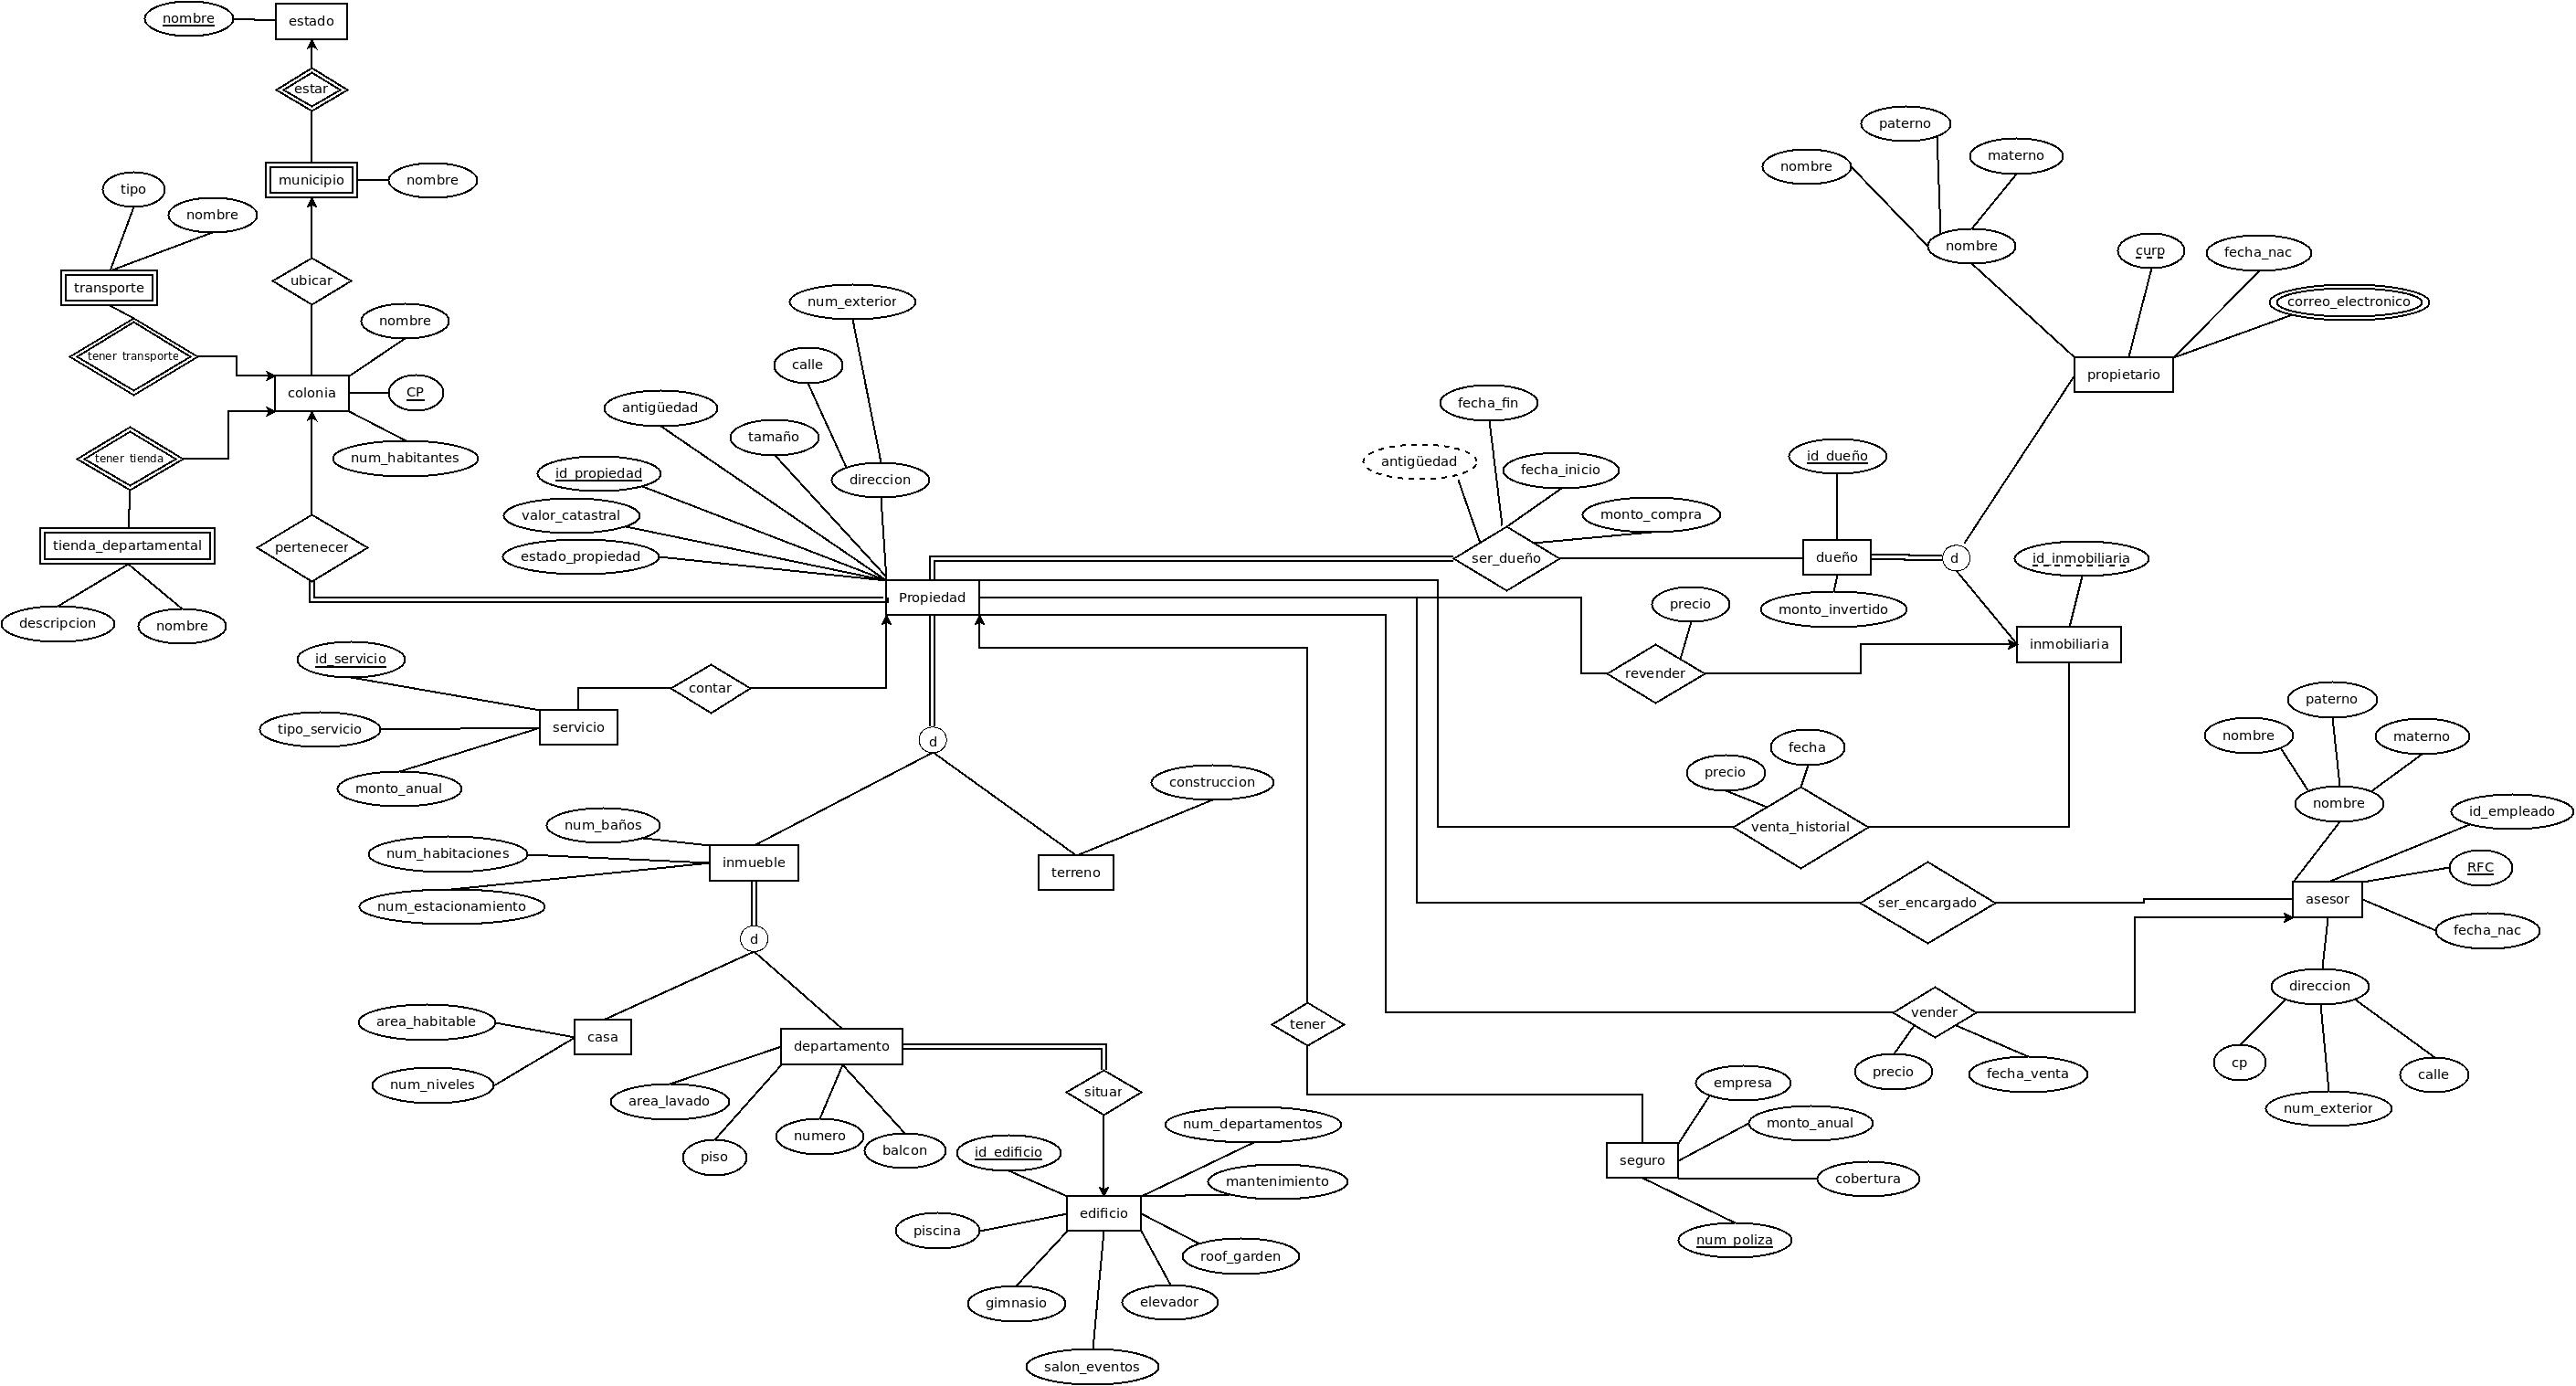
\includegraphics[width=1cm]{modeloER}}
\rhead[CAPÍTULO \thechapter. \leftmark]{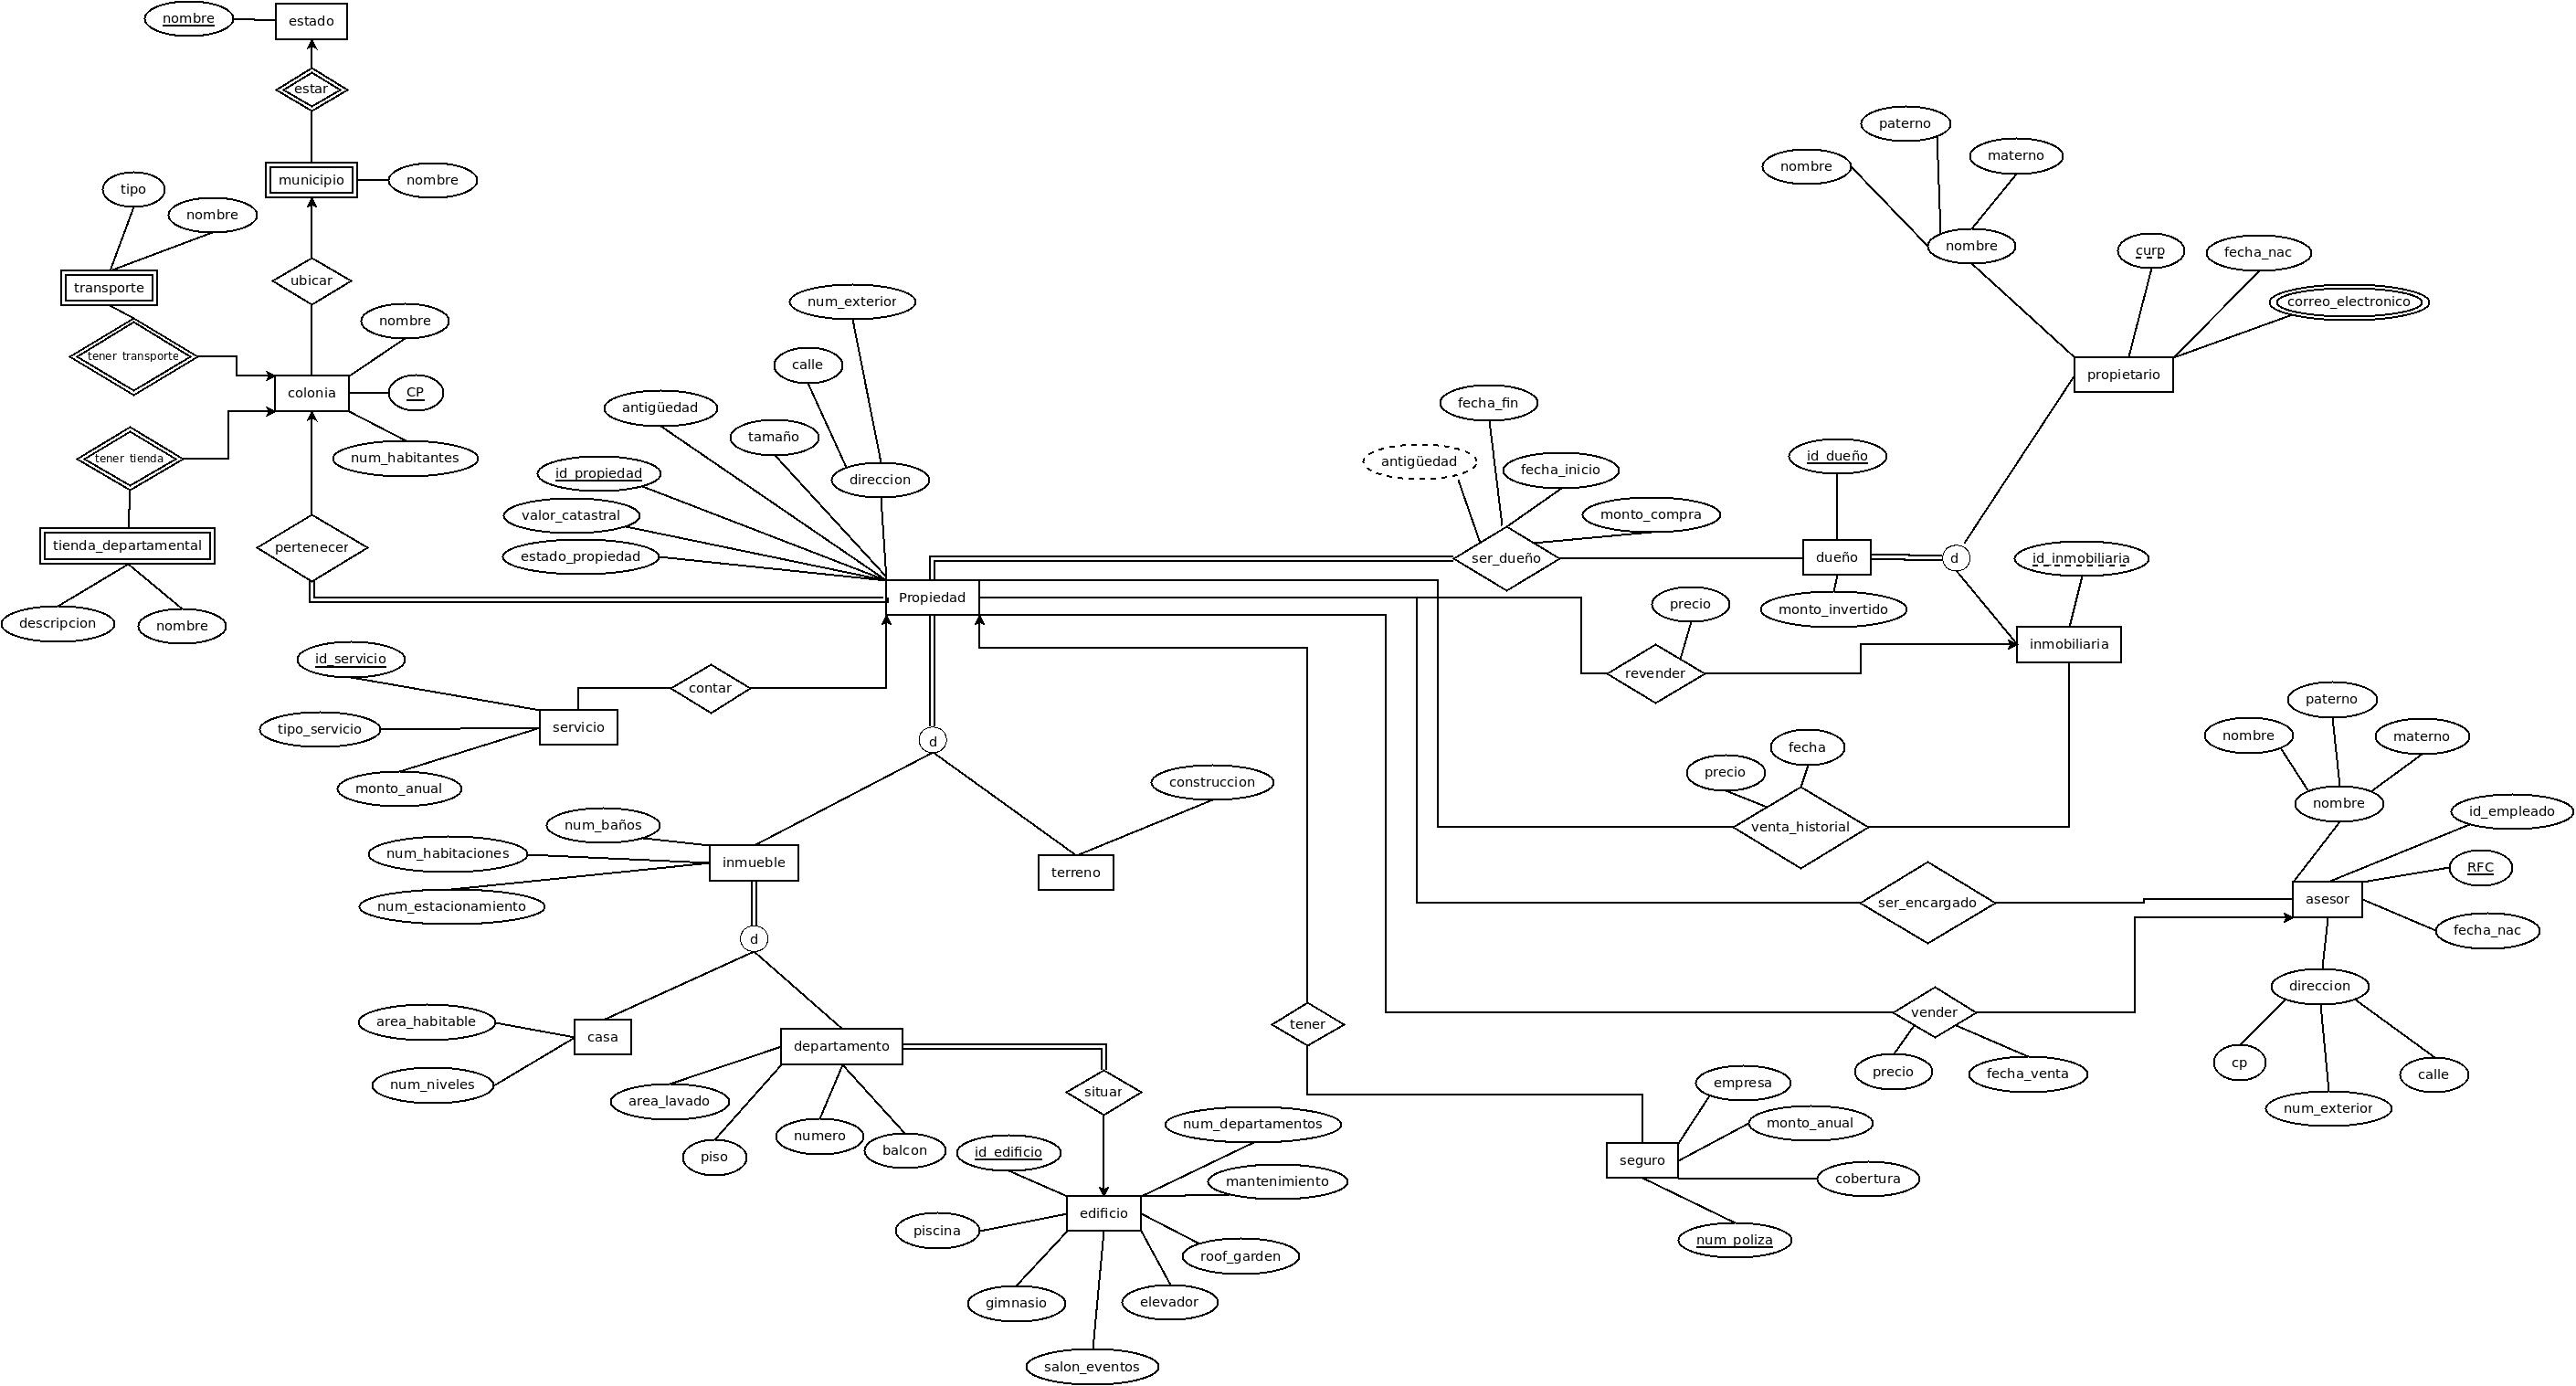
\includegraphics[width=1cm]{modeloER}}

%\chapter{Introducción}\label{cap.intro}
%\markboth{INTRODUCCIÓN}{INTRODUCCIÓN}

Bla bla bla...

\section{Estado del Arte}

%\lhead[\thepage]{\thesection. Estado del Arte}

Bla bla bla...

\section{Objetivos de la Tesis}
%\lhead[\thepage]{\thesection. Objetivos de la Tesis}

Bla bla bla...

%\chapter{Nudo}\label{cap.nudo}
%\markboth{NUDO}{NUDO}

Bla bla bla...

\section{Situación Mundial}
%\lhead[\thepage]{\thesection. Situación Mundial}

Bla bla bla...

\end{document}